% Combined Q1--Q2 manuscript.
\documentclass[11pt,a4paper]{article}

\usepackage[a4paper,top=2.4cm,bottom=2.3cm,left=2.35cm,right=2.35cm,footskip=1.1cm]{geometry}
\usepackage{iftex}
\ifPDFTeX
  \usepackage[T1]{fontenc}
  \usepackage[utf8]{inputenc}
  \usepackage{newtxtext,newtxmath}
\else
  \usepackage{fontspec}
  \setmainfont{TeX Gyre Termes}
  \usepackage{unicode-math}
  \setmathfont{TeX Gyre Termes Math}
\fi
\usepackage{graphicx}
\usepackage{xcolor}
\usepackage{booktabs,tabularx,array,multirow,longtable}
\usepackage{enumitem}
\usepackage{microtype}
\usepackage{caption}
\usepackage{subcaption}
\usepackage{float}
\usepackage{fancyhdr}
\usepackage{titlesec}
\usepackage{tikz}
\usetikzlibrary{arrows.meta,positioning,shapes.geometric}
\usepackage[hidelinks]{hyperref}

\definecolor{Ink}{HTML}{18324A}
\definecolor{Accent}{HTML}{197C83}
\definecolor{Pale}{HTML}{EAF2F4}
\setlength{\parindent}{1.5em}
\setlength{\parskip}{0.15em}
\setlength{\emergencystretch}{2em}
\renewcommand{\baselinestretch}{1.08}
\setcounter{secnumdepth}{3}
\captionsetup{font=small,labelfont=bf,labelsep=period,skip=5pt}
\captionsetup[subfigure]{justification=raggedright,singlelinecheck=false}
\titleformat{\section}{\large\bfseries\color{Ink}}{\thesection}{0.65em}{}
\titleformat{\subsection}{\normalsize\bfseries\color{Ink}}{\thesubsection}{0.6em}{}
\titleformat{\subsubsection}{\normalsize\bfseries}{\thesubsubsection}{0.6em}{}
\titlespacing*{\section}{0pt}{1.2em}{0.45em}
\titlespacing*{\subsection}{0pt}{0.85em}{0.3em}
\titlespacing*{\subsubsection}{0pt}{0.6em}{0.2em}
\pagestyle{fancy}
\fancyhf{}
\fancyhead[L]{\small\color{Ink}UAV EMERGENCY SUPPLY PLANNING}
\fancyhead[R]{\small\thepage}
\renewcommand{\headrulewidth}{0.35pt}
\renewcommand{\headrule}{\hbox to\headwidth{\color{Accent}\leaders\hrule height \headrulewidth\hfill}}
\setlength{\headheight}{22pt}
\renewcommand{\topfraction}{0.88}
\renewcommand{\bottomfraction}{0.72}
\renewcommand{\textfraction}{0.12}
\renewcommand{\floatpagefraction}{0.78}
\setcounter{topnumber}{3}
\setcounter{bottomnumber}{2}
\setcounter{totalnumber}{5}
\setlength{\textfloatsep}{10pt plus 2pt minus 2pt}
\setlength{\intextsep}{9pt plus 2pt minus 2pt}

\newcommand{\Ehor}{E^{\mathrm{hor}}}
\newcommand{\Eup}{E^{\mathrm{up}}}
\newcommand{\ND}{\operatorname{ND}}
\newcommand{\SOC}{\mathrm{SOC}}
\newcommand{\kWh}{\,\mathrm{kWh}}
\newcommand{\kg}{\,\mathrm{kg}}
\newcommand{\m}{\,\mathrm{m}}
\newcommand{\s}{\,\mathrm{s}}
\newcommand{\keywords}[1]{\par\noindent\textbf{Keywords:} #1}
\begin{document}
\pagenumbering{gobble}
\begin{titlepage}
\thispagestyle{empty}
\centering
\vspace*{0.45cm}
\begin{tabular}{@{}c@{\hspace{0.35cm}}c@{\hspace{0.35cm}}c@{}}
  
\includegraphics[width=82pt,height=53pt,keepaspectratio]{figs/cpipc-logo.png} &
  
\includegraphics[width=64pt,height=62pt,keepaspectratio]{figs/contest-logo.png} &
  
\includegraphics[width=66pt,height=66pt,keepaspectratio]{figs/huawei-logo.png}\\
\end{tabular}\par
\vspace{1.05cm}
{\large\sffamily\bfseries\color{Ink}China Postgraduate Innovation \& Practice Competitions\par}
\vspace{0.35cm}
{\Large\sffamily\bfseries\color{Ink}The 23rd “Huawei Cup” China Post-Graduate\\[-0.05em]
Mathematical Contest in Modeling\par}
\vspace{0.9cm}
{\LARGE\bfseries\color{Ink}Terrain-Aware Routing and Fleet Scheduling for UAV Emergency Supply\par}
\vspace{0.2cm}
{\large\color{Ink}Terrain-Constrained Cargo Batching and Multi-Stop Fleet Scheduling\par}
\vspace{0.9cm}
\begin{minipage}{0.88\linewidth}
\centering
\renewcommand{\arraystretch}{1.35}
\begin{tabular}{@{}p{3.3cm}p{10cm}@{}}
\textbf{University} & \hrulefill\\ \hline
\textbf{Team Number} & \hrulefill\\ \hline
\multirow{3}{3.3cm}{\centering\textbf{Team Members}} & 1.\ \hrulefill\\
 & 2.\ \hrulefill\\
 & 3.\ \hrulefill\\ \hline
\end{tabular}
\end{minipage}
\end{titlepage}
\pagenumbering{arabic}

\begin{abstract}
We study terrain-constrained cargo batching and multi-stop fleet scheduling for UAV emergency supply. For the first task, exhaustive feasible-batch generation and subset dynamic programming produce the complete baseline Pareto set; its representative plan uses 18 sorties, while the minimum-energy endpoint uses 19. For the second task, adaptive large-neighborhood search with deadline-directed route enrichment and tabu-guided neighborhood search yields a feasible 24-sortie schedule, compared with 39 sorties for the late-first baseline. The recommendation meets all hard deadlines and resource constraints. An 18-sortie route-cover lower bound applies to the initial candidate pool, but the full scheduling problem is not certified optimal. Energy results depend on the stated flight-energy model.
\end{abstract}
\keywords{UAV logistics; terrain-aware routing; multiobjective optimization; fleet scheduling; adaptive large-neighborhood search}

\section{Question 1: Terrain-Constrained UAV Cargo Batching}
\subsection{Problem and data}
\subsubsection{Mathematical restatement}
Let $S=\{1,\ldots,15\}$ be the service areas, $C_s$ the cargo boxes assigned to area $s$, and $G=\{A,B,C\}$ the aircraft models. A sortie chooses one area $s$, one aircraft model $g$, and one nonempty subset $B\subseteq C_s$. It flies depot $O01\to s$, transfers all boxes in $B$, and returns $s\to O01$ without cargo. Every box is delivered once; boxes are not split or mixed across service areas. The objectives are to minimize the total number of sorties $N$, total modeled energy $E$, and total cumulative operating time $T$.

The 80 boxes weigh 758 kg in total and occupy 2.011 m$^3$. Each of the 15 areas has 3--15 boxes. Table~\ref{tab:aircraft} gives the aircraft payload and volume limits. The continuous payload bound is determined by the return-energy reserve. Range and batch-volume limits are checked separately for each selected batch.

\begin{table}[H]
\centering
\caption{Nominal aircraft loading limits used in Q1.}
\label{tab:aircraft}
\begin{tabular}{lrr}
\toprule
Aircraft model & Maximum cargo mass (kg) & Loading volume (m$^3$)\\
\midrule
A & 25 & 0.060\\
B & 30 & 0.073\\
C & 80 & 0.250\\
\bottomrule
\end{tabular}
\end{table}

Figures~\ref{fig:q1-mass-volume} and~\ref{fig:q1-area-demand} show the two input features that shape batch feasibility: box mass and volume, and demand by service area.

\begin{figure}[H]\centering
\includegraphics[width=0.55\linewidth,height=0.68\textheight,keepaspectratio]{figs/q1_fig02_mass_volume.pdf}\caption{Mass--volume pairs for the 80 boxes, grouped by cargo class.}\label{fig:q1-mass-volume}\end{figure}
\begin{figure}[H]\centering
\includegraphics[width=0.55\linewidth,height=0.68\textheight,keepaspectratio]{figs/q1_fig03_area_demand.pdf}\caption{Exact number of cargo boxes assigned to each service area; all 15 areas are shown.}\label{fig:q1-area-demand}\end{figure}

\subsubsection{Input processing and scope}
Cargo records are checked for unique IDs, valid mass and volume, and complete area coverage. Coordinates are projected to a local metric system. Each straight flight segment is sampled against intersected cells of the 30-m digital elevation model (DEM), and the maximum elevation sets its cruise altitude. Segments outside the DEM domain or crossing NoData are excluded from the candidate set.

\subsection{Physical feasibility model}
\subsubsection{Terrain, range, and flight time}
For a directed leg $i\to j$, let $d_{ij}$ denote the projected horizontal distance and $z^{\max}_{ij}$ the maximum DEM elevation along the straight horizontal route. The specified cruise altitude and climb/descent increments are
\begin{align}
z^{\mathrm{cr}}_{ij}&=z^{\max}_{ij}+50\m,\\
h^+_{ij}&=\max\{0,z^{\mathrm{cr}}_{ij}-z_i^{\mathrm{op}}\},\qquad
h^-_{ij}=\max\{0,z^{\mathrm{cr}}_{ij}-z_j^{\mathrm{op}}\},
\end{align}
where the depot operates at its supplied elevation and a service-area aircraft operates 30 m above its supplied elevation. For aircraft model $g$, the payload-dependent range $L_g(q)$ and leg time $t_{gij}$ follow the supplied range and speed relationships:
\begin{align}
L_g(q)&=L_g^0-(L_g^0-L_g^F)\left(\frac{q}{Q_g}\right)^{3/2},\quad 0\le q\le Q_g,\label{eq:range}\\
t_{gij}&=\frac{h^+_{ij}}{v_g^\uparrow}+\frac{d_{ij}}{v_g^c}+\frac{h^-_{ij}}{v_g^\downarrow}.\label{eq:time}
\end{align}
Here $Q_g$ is rated payload, $L_g^0,L_g^F$ are unloaded and fully loaded ranges, and $v_g^\uparrow,v_g^c,v_g^\downarrow$ are climb, cruise, and descent speeds.

\subsubsection{Conditional energy convention}
The task separates horizontal and ascent energy but does not specify their equations. We model these components as
\begin{align}
\Ehor_{gij}(q)&=E_g^{\mathrm{use}}\frac{d_{ij}}{L_g(q)},\\
\Eup_{gij}(q)&=\frac{(M_g+q)g h^+_{ij}}{3.6\times10^6\eta_g^\uparrow},\\
E_{gij}(q)&=\Ehor_{gij}(q)+\Eup_{gij}(q),
\label{eq:energy}
\end{align}
where $E_g^{\mathrm{use}}$ is usable battery energy, $M_g$ is empty aircraft mass, $g=9.81\ \mathrm{m\,s^{-2}}$, and $\eta_g^\uparrow$ is climb efficiency. The horizontal term scales with distance relative to payload-adjusted range; the ascent term is gravitational potential energy converted to kWh. Descent energy is omitted. All energy results therefore depend on this convention and the specified usable-energy values.

For a cargo subset $B$ with total mass $m(B)$, the outbound leg carries $m(B)$ and the return leg is empty. Let $\SOC$ denote the state of charge. Then
\begin{equation}
E_{gsB}=E_{g,O01,s}(m(B))+E_{g,s,O01}(0),\qquad
\SOC^{\mathrm{return}}_{gsB}=1-\frac{E_{gsB}}{E_g^{\mathrm{use}}}\ge \rho_g.
\label{eq:roundtrip}
\end{equation}
Range is checked separately by $d_{O01,s}/L_g(m(B))+d_{s,O01}/L_g(0)\le1$. The continuous safe payload is
\begin{equation}
q^{\max}_{gs}=\max\{q\in[0,Q_g]: E_{g,O01,s}(q)+E_{g,s,O01}(0)\le(1-\rho_g)E_g^{\mathrm{use}}\}.
\label{eq:qmax}
\end{equation}
If an empty round trip violates the reserve, $(g,s)$ is unreachable. Actual cargo batches must also satisfy the rated mass and volume limits; volume does not enter Eq.~\eqref{eq:qmax}.

The baseline reserve is $\rho=0.20$. We test model sensitivity by scaling horizontal and ascent energy by $\alpha,\beta\in\{0.9,1.0,1.1\}$ and re-solving at reserves $\rho\in\{0.20,0.30,0.40\}$. 

\subsection{Discrete batching and objectives}
\subsubsection{Feasible candidate set}
For each area, every nonempty cargo subset is paired with each of the three aircraft types. Candidate $b=(s,g,B)$ is retained only if
\begin{equation}
m(B)\le Q_g,\qquad v(B)\le V_g,\qquad
E_{gsB}\le(1-\rho_g)E_g^{\mathrm{use}},\qquad
\frac{d_{O01,s}}{L_g(m(B))}+\frac{d_{s,O01}}{L_g(0)}\le1.
\label{eq:candidate}
\end{equation}
No candidate cap is imposed. Since $|C_s|\le15$, area-wise exhaustive enumeration is bounded by $3(2^{|C_s|}-1)$ model--subset pairs before physical pruning.

Let $x_b\in\{0,1\}$ indicate selection of candidate $b$, and $C_b$ its box set. The exact set-partitioning requirements are
\begin{equation}
\sum_{b:c\in C_b}x_b=1\quad(\forall c\in C),\qquad x_b\in\{0,1\}.
\label{eq:partition}
\end{equation}
This equality enforces both complete delivery and no duplicate delivery. For each sortie, the modeled operating time includes round-trip flight, baseline handover, per-box handover, preflight preparation, and per-box loading:
\begin{equation}
T_b=t_{g,O01,s}+t_{g,s,O01}+t_g^{\mathrm{prep}}+|C_b|t_g^{\mathrm{load}}+t_g^{\mathrm{hand,base}}+|C_b|t_g^{\mathrm{hand,box}}.
\label{eq:batchtime}
\end{equation}
We minimize the vector
\begin{equation}
\min\;(F_N,F_E,F_T)=\left(\sum_bx_b,\ \sum_bE_bx_b,\ \sum_bT_bx_b\right).
\label{eq:objectives}
\end{equation}
$F_T$ is cumulative operating time summed over sorties. Q1 assigns no individual airframes and models no parallel execution, so it is not a fleet makespan and should not be interpreted as elapsed wall-clock completion time.

\subsubsection{Exact subset dynamic programming}
For area $s$ and local cargo subset $U\subseteq C_s$, let $P_s(U)$ contain the nondominated triples $(N,E,T)$ and their realizing partitions. Set $P_s(\varnothing)=\{(0,0,0)\}$. For nonempty $U$, let $i(U)$ be its lowest-indexed box and consider only feasible batches containing it:
\begin{equation}
P_s(U)=\ND\left\{(1,E_b,T_b)+p:\ b\in\mathcal B_s,\ C_b\subseteq U,\ i(U)\in C_b,\ p\in P_s(U\setminus C_b)\right\}.
\label{eq:dp}
\end{equation}
Anchoring every transition at the lowest uncovered box generates each partition once. At a fixed coverage mask, a dominated partial objective vector can be discarded: any continuation adds the same feasible future batch vectors, and therefore cannot make the dominated vector nondominated. After each area's full set has been solved, area fronts are combined by Minkowski addition and Pareto pruning:
\begin{equation}
\mathcal P=\ND\left(P_1(C_1)\oplus P_2(C_2)\oplus\cdots\oplus P_{15}(C_{15})\right).
\label{eq:merge}
\end{equation}
The decomposition is valid because Q1 has no shared aircraft, battery, charging, or inter-area timing constraints. Exactness is with respect to the fully enumerated candidates and the recorded floating-point comparison tolerances. This recurrence follows the established use of dynamic programming for discrete multicriteria optimization, while the area-wise state decomposition is tailored to this instance \cite{carraway1990,ehrgott2000}.

Figure~\ref{fig:q1-workflow} summarizes the sequence from physical screening to the exact Pareto set and plan selection.

\begin{figure}[H]
\centering
\begin{tikzpicture}[
  node distance=0.48cm,
  processbox/.style={draw=Accent,rounded corners=2pt,fill=Pale,align=center,text width=0.78\linewidth,minimum height=0.62cm,font=\small},
  arr/.style={-{Stealth[length=2mm]},thick,color=Accent}]
  \node[processbox] (data) {Cargo, aircraft, depot/service-area coordinates, and 30-m DEM};
  \node[processbox,below=of data] (physics) {Terrain profile, loaded-outbound / empty-return range and conditional energy};
  \node[processbox,below=of physics] (enum) {Enumerate area batches; check payload, volume, range, and reserve};
  \node[processbox,below=of enum] (dp) {Exact subset DP per area; prune dominated states at equal coverage};
  \node[processbox,below=of dp] (merge) {Minkowski merge of 15 area fronts and global nondominance pruning};
  \node[processbox,below=of merge] (report) {Scenario feasibility, Pareto set, and representative plan};
  \draw[arr] (data)--(physics); \draw[arr] (physics)--(enum); \draw[arr] (enum)--(dp); \draw[arr] (dp)--(merge);
  \draw[arr] (merge)--(report);
\end{tikzpicture}
\caption{Q1 workflow from terrain-aware feasibility checks to exact multiobjective batching.}
\label{fig:q1-workflow}
\end{figure}

\subsubsection{Pareto interpretation and representative plan}
A solution dominates another if it is no worse in all three objectives and strictly better in at least one. We retain the complete nondominated set rather than imposing an arbitrary scalar trade-off during optimization. For descriptive comparison, each objective's ideal value $L_j$ and nadir value $U_j$ are computed from the complete front. The representative plan minimizes its equal-weight Euclidean distance to the normalized ideal:
\begin{equation}
\widehat F_j(x)=\begin{cases}(F_j(x)-L_j)/(U_j-L_j),&U_j>L_j,\\0,&U_j=L_j,\end{cases}\qquad
x^{\mathrm{rep}}=\arg\min_{x\in\mathcal P}\sqrt{\sum_{j\in\{N,E,T\}}\widehat F_j(x)^2}.
\label{eq:representative}
\end{equation}
Ties within numerical tolerance are resolved by sortie count, energy, cumulative time, and canonical plan ID.

\subsection{Computational procedure and verification}
For every reported partition, we independently recompute cargo coverage, mass and volume, loaded-outbound/empty-return range, energy reserve, flight time, and objective totals. All 27 sensitivity scenarios were resolved: 18 have feasible complete fronts, while nine have no feasible partition.

Figure~\ref{fig:q1-candidate-reduction} shows how physical screening and dominance pruning reduce the initial model--subset combinations.

\begin{figure}[H]\centering
\includegraphics[width=0.55\linewidth,height=0.68\textheight,keepaspectratio]{figs/q1_fig04_candidate_reduction.pdf}\caption{Candidate counts after each screening stage across the 27 scenarios. The line and band show the median and interquartile range; the vertical axis is logarithmic.}\label{fig:q1-candidate-reduction}\end{figure}
\subsection{Results and discussion}
\subsubsection{Safe payload and baseline feasibility}
At the baseline $(\rho,\alpha,\beta)=(0.20,1,1)$, the 45 aircraft--area pairs include 15 A pairs capped by the 25-kg rating, 14 B pairs capped at 30 kg, and 10 C pairs capped at 80 kg. The remaining six are limited by energy. Figure~\ref{fig:q1-capacity} shows the energy-limited payload bound; actual batches also satisfy range and volume limits.

\begin{figure}[H]\centering
\includegraphics[width=0.98\linewidth,height=0.45\textheight,keepaspectratio]{figs/q1_fig07_capacity_envelope.pdf}\caption{Energy-limited payload (kg) under the baseline return reserve for each aircraft--area pair. Range and volume are checked separately. Color and cell annotations show the same value; an em dash marks an unreachable pairing.}\label{fig:q1-capacity}\end{figure}

A feasible partition exists for all nine $(\alpha,\beta)$ combinations at $\rho=0.20$, six at $\rho=0.30$, and three at $\rho=0.40$. Figure~\ref{fig:q1-front-cardinality} gives the size of each exact Pareto front; X marks a scenario with no feasible partition.
\begin{figure}[H]\centering
\includegraphics[width=0.98\linewidth,height=0.45\textheight,keepaspectratio]{figs/q1_fig06_frontier_cardinality.pdf}\caption{Cardinality of the complete exact nondominated objective set for each reserve and energy-multiplier combination. X marks a proven-infeasible scenario.}\label{fig:q1-front-cardinality}\end{figure}

\subsubsection{Exact baseline trade-off}
The baseline Pareto front has two objective vectors (Table~\ref{tab:baseline}). The representative uses 18 sorties and minimizes both sortie count and cumulative time; the 19-sortie endpoint uses the least energy. Under Eq.~\eqref{eq:representative}, the representative uses 0.09736 kWh (0.165\%) more energy and saves 1,663.973 s. 

\begin{table}[H]
\centering
\caption{Complete baseline Pareto front and selected representative.}
\label{tab:baseline}
\begin{tabularx}{\linewidth}{@{}lrrr>{\raggedright\arraybackslash}X@{}}
\toprule
Plan & Sorties & Energy (kWh) & Cumulative time (s) & Interpretation\\
\midrule
Representative & 18 & 59.131669 & 32,776.093 & Equal-weight normalized ideal-distance rule; fewer sorties\\
Minimum-energy endpoint & 19 & 59.034314 & 34,440.065 & Lowest energy on the complete front\\
\bottomrule
\end{tabularx}
\end{table}


The representative uses nine model-B sorties and nine model-C sorties. Figure~\ref{fig:q1-manifest} shows their cargo-class composition. Each B sortie carries 25 kg and together they deliver 27 boxes; C sorties carry 45--78 kg (mean 59.22 kg) and deliver the remaining 53. Each of the 80 boxes appears once.

\begin{figure}[H]\centering
\includegraphics[width=0.98\linewidth,height=0.58\textheight,keepaspectratio]{figs/q1_fig09_sortie_manifest.pdf}\caption{Cargo-class mass composition (kg) of the 18 representative sorties, grouped by aircraft model. Each stack gives one sortie's payload.}\label{fig:q1-manifest}\end{figure}

\subsubsection{Reserve and energy sensitivity}
Each sensitivity case is fully re-enumerated and re-optimized. Figure~\ref{fig:q1-sensitivity} shows the representative's energy change from baseline; X marks cases with no feasible partition. Higher reserve requirements can make the complete assignment infeasible.

\begin{figure}[H]\centering
\includegraphics[width=0.98\linewidth,height=0.45\textheight,keepaspectratio]{figs/q1_fig10_energy_sensitivity.pdf}\caption{Change in selected representative total energy (kWh) from baseline over the reserve and energy-multiplier grid. Each feasible cell is fully re-solved; X denotes a proven-infeasible scenario.}\label{fig:q1-sensitivity}\end{figure}

The full sensitivity results show when re-optimization changes the selected plan, not only its energy. At $\rho=0.20$, six scenarios retain the baseline 18-sortie partition with no changed batch pairs; the remaining three use 19 or 21 sorties and change 3--7 batch pairs. At $\rho=0.30$, the three $\alpha=0.9$ cases retain the baseline partition, while the three $\alpha=1.0$ cases use 22 sorties and change 16 batch pairs. At $\rho=0.40$, the three feasible cases use 23 or 25 sorties and change 19--21 batch pairs. The nine infeasible scenarios are the three $\alpha=1.1$ cases at $\rho=0.30$ and all six cases with $\alpha\in\{1.0,1.1\}$ at $\rho=0.40$; they have no representative-plan deltas. Table~\ref{tab:q1-sensitivity-details} reports the feasible-case changes in sorties, energy, cumulative operating time, and aircraft--batch assignments.

\begin{table}[H]
\centering\scriptsize
\caption{Representative-plan changes under each feasible reserve and energy-multiplier scenario, relative to the baseline. Batch-pair changes count changed aircraft--cargo-batch assignments. Values are shown to three decimals.}
\label{tab:q1-sensitivity-details}
\begin{tabular}{@{}rrrrrrr@{}}
\toprule
$\rho$ & $\alpha$ & $\beta$ & $\Delta N$ & $\Delta E$ (kWh) & $\Delta T$ (s) & Changed batch pairs\\
\midrule
0.20 & 0.9 & 0.9 & 0 & -5.913 & 0.000 & 0\\
0.20 & 0.9 & 1.0 & 0 & -5.658 & 0.000 & 0\\
0.20 & 0.9 & 1.1 & 0 & -5.402 & 0.000 & 0\\
0.20 & 1.0 & 0.9 & 0 & -0.256 & 0.000 & 0\\
0.20 & 1.0 & 1.0 & 0 & 0.000 & 0.000 & 0\\
0.20 & 1.0 & 1.1 & 0 & +0.256 & 0.000 & 0\\
0.20 & 1.1 & 0.9 & 1 & +7.517 & +1789.648 & 3\\
0.20 & 1.1 & 1.0 & 3 & +9.978 & +5235.463 & 7\\
0.20 & 1.1 & 1.1 & 3 & +10.261 & +5235.463 & 7\\
0.30 & 0.9 & 0.9 & 0 & -5.913 & 0.000 & 0\\
0.30 & 0.9 & 1.0 & 0 & -5.658 & 0.000 & 0\\
0.30 & 0.9 & 1.1 & 0 & -5.402 & 0.000 & 0\\
0.30 & 1.0 & 0.9 & 4 & +7.437 & +7023.725 & 16\\
0.30 & 1.0 & 1.0 & 4 & +7.727 & +7023.725 & 16\\
0.30 & 1.0 & 1.1 & 4 & +8.018 & +7023.725 & 16\\
0.40 & 0.9 & 0.9 & 5 & +7.149 & +9126.139 & 19\\
0.40 & 0.9 & 1.0 & 5 & +7.453 & +9126.139 & 19\\
0.40 & 0.9 & 1.1 & 7 & +9.519 & +12700.917 & 21\\
\bottomrule
\end{tabular}
\end{table}

\subsubsection{Limitations}
The energy equations are modeling assumptions because the task does not specify the component formulas. The sensitivity analysis shows how results change under nearby energy and reserve settings but cannot replace calibration against flight data. Routes use straight segments and static terrain elevation; wind, weather, turning, and battery aging are not modeled. Q1 sums sortie operating times without assigning aircraft or allowing parallel flights, so its time objective is not a fleet makespan.

\section{Question 2: Joint Scheduling of Multi-Destination UAV Sorties}
\subsection{Problem and data}
Question 2 extends Q1's single-area batches to multi-stop sorties that return to O01. Each sortie specifies its cargo, stop sequence, aircraft, drone, battery, and preparation time. The instance has 80 boxes across 15 areas, including 30 initial-delivery boxes. Every box must be delivered once. Medical boxes must meet their desired times; initial-delivery boxes must meet their stated deadlines. Other desired times contribute to the lateness objective but are not hard constraints.

Let $\mathcal C$ be the cargo set, $m_c$ and $v_c$ the mass and volume of box $c$, $D_c^{\mathrm{des}}$ its desired delivery time, $D_c^{\mathrm{init}}$ its initial-delivery deadline when applicable, and $w_c$ its priority weight. Figure~\ref{fig:q2-mass-volume} groups mass--volume pairs by priority; Figure~\ref{fig:q2-desired-times} shows the requested delivery-time distribution. The fleet has eight drones (four A, two B, and two C) and 6, 4, and 4 shared batteries for models A, B, and C; battery counts include mounted batteries.

\begin{figure}[H]\captionsetup{justification=raggedright,singlelinecheck=false}\centering\includegraphics[width=0.75\linewidth]{figs/q2_raw_q2_mass_volume_priority.pdf}\caption{Box mass and volume by priority. Bubble area is proportional to the number of boxes at each mass--volume pair; labels give exact counts.}\label{fig:q2-mass-volume}\end{figure}
\begin{figure}[H]\captionsetup{justification=raggedright,singlelinecheck=false}\centering\includegraphics[width=0.75\linewidth]{figs/q2_raw_q2_desired_windows.pdf}\caption{Frequency of requested delivery times for the 80 boxes.}\label{fig:q2-desired-times}\end{figure}

\subsection{Candidate routes and physical feasibility}
Let $\mathcal R$ be the candidate route pool. Each route $p$ fixes its aircraft model $g_p$, cargo set $C_p$, stop-level deliveries $C_{p,k}$, and sequence $O01\to v_{p,1}\to\cdots\to v_{p,h_p}\to O01$. Each stop delivers at least one box to its service area; an area may appear at multiple stops. Q1 batches and feasible single-box sorties seed the pool. Insertion, migration, exchange, stop changes, and disjoint-route merges generate additional routes. The initial pool contains 400 routes per aircraft model; deadline-directed enrichment expands it to 2,628 routes.

For each leg $(i,j)$ of route $p$, let $q_{p,ij}$ be the mass still aboard before departure. Its load decreases after each handover and is zero on the return leg. With model limits $Q_g$ and $V_g$, route energy $E_p$, usable battery energy $E_g^{\mathrm{use}}$, and return reserve $\rho_g$, physical feasibility requires
\begin{equation}
q_{p,ij}\le Q_{g_p},\qquad \sum_{c\in C_p}v_c\le V_{g_p},\qquad E_p=\sum_{(i,j)\in p}E_{g_p,ij}(q_{p,ij})\le(1-\rho_{g_p})E_{g_p}^{\mathrm{use}}.
\label{eq:q2-physics}
\end{equation}
Each route must also satisfy the payload-adjusted range limit
\begin{equation}
\sum_{(i,j)\in p}\frac{d_{ij}}{L_{g_p}(q_{p,ij})}\le1.
\label{eq:q2-range}
\end{equation}
Before scheduling, each route has a preparation and loading duration $P_p$, delivery offsets $\tau_{p,c}$ from takeoff, a return time $\tau_p^{\mathrm{return}}$, and return state of charge $r_p$. Full-recharge time follows the two-phase charging rule, $T_p^{\mathrm{chg}}=t_{g_p}^{\mathrm{full}}f(r_p)$, with $f(r)=0.65(0.90-r)/0.90+0.35$ for $r<0.90$ and $f(r)=0.35(1-r)/0.10$ otherwise. Figures~\ref{fig:q2-pool-model} and~\ref{fig:q2-stop-counts} summarize the initial route pool.

\begin{figure}[H]\centering
\begin{subfigure}[t]{0.49\linewidth}\centering
\includegraphics[width=0.98\linewidth]{figs/q2_process_q2_pool_by_model.pdf}
\caption{Generated proposals and retained routes by aircraft model in the initial 400-route-per-model pool.}\label{fig:q2-pool-model}
\end{subfigure}\hfill
\begin{subfigure}[t]{0.49\linewidth}\centering
\includegraphics[width=0.98\linewidth]{figs/q2_process_q2_route_stop_counts.pdf}
\caption{Candidate-route counts by stop count in the initial pool.}\label{fig:q2-stop-counts}
\end{subfigure}
\end{figure}

\subsection{Joint schedule and search objectives}
Each selected route receives a compatible drone, a battery, and a preparation start $s_p\ge0$. The selection and assignment constraints are
\begin{equation}
\sum_{p:c\in C_p}x_p=1\quad(c\in\mathcal C),\qquad
\sum_{u\in\mathcal U_{g_p}}y_{pu}=x_p,\qquad
\sum_{b\in\mathcal B_{g_p}}z_{pb}=x_p,
\label{eq:q2-cover}
\end{equation}
where $x_p,y_{pu},z_{pb}$ denote route selection, drone assignment, and battery assignment. Let $\mathcal C^{\mathrm{med}}$ and $\mathcal C^{\mathrm{init}}$ denote medical and initial-delivery boxes. For the selected route $p$ carrying $c$, the delivery time and hard deadlines satisfy
\begin{equation}
d_c=s_p+P_p+\tau_{p,c}\quad(x_p=1,\ c\in C_p),\quad d_c\le D_c^{\mathrm{des}}\ (c\in\mathcal C^{\mathrm{med}}),\quad d_c\le D_c^{\mathrm{init}}\ (c\in\mathcal C^{\mathrm{init}}).
\label{eq:q2-deadlines}
\end{equation}
\begin{samepage}
A drone is occupied from preparation through return, for $D_p^U=P_p+\tau_p^{\mathrm{return}}$; turnaround time is zero. Battery occupancy also includes full recharge, $D_p^B=D_p^U+T_p^{\mathrm{chg}}$. Two routes assigned to the same resource must have disjoint occupancy intervals:
\begin{align}
[s_p,s_p+D_p^U)\cap[s_q,s_q+D_q^U)&=\varnothing &&(p<q,\ u\in\mathcal U_{g_p}\cap\mathcal U_{g_q},\ y_{pu}=y_{qu}=1),\label{eq:q2-drone-nonoverlap}\\
[s_p,s_p+D_p^B)\cap[s_q,s_q+D_q^B)&=\varnothing &&(p<q,\ b\in\mathcal B_{g_p}\cap\mathcal B_{g_q},\ z_{pb}=z_{qb}=1).\label{eq:q2-battery-nonoverlap}
\end{align}
These disjunctions are represented by binary precedence variables in the MILP cross-check. A battery can serve any compatible drone of the same model. Makespan ends when the last drone returns and excludes recharge.\end{samepage}
For each box, $\ell_c\ge\max(0,d_c-D_c^{\mathrm{des}})$. The four minimization objectives are
\begin{align}
F_{\mathrm{late}}&=\sum_{c\in\mathcal C}w_c\ell_c, &
F_{\mathrm{makespan}}&=\max_{p:x_p=1}(s_p+P_p+\tau_p^{\mathrm{return}}),\\
F_{\mathrm{energy}}&=\sum_{p\in\mathcal R}E_px_p, &
F_{\mathrm{sortie}}&=\sum_{p\in\mathcal R}x_p.
\label{eq:q2-objectives}
\end{align}
Weighted lateness is measured in priority-seconds. The late-first baseline prioritizes weighted lateness, then makespan, energy, and sortie count. The recommended search prioritizes sortie count, then weighted lateness, makespan, and energy. We solve the full instance with adaptive large-neighborhood search (ALNS), deadline-directed route enrichment, and tabu-guided variable-neighborhood search (VNS). A small exact mixed-integer linear program (MILP) instance checks the constraint implementation. The reported archive contains schedules found by this search. Table~\ref{tab:q2-notation} summarizes the principal symbols.

Figure~\ref{fig:q2-workflow} summarizes the search. Figure~\ref{fig:q2-drone-schedule} shows drone occupancy in the recommended schedule. Figure~\ref{fig:q2-heuristic-archive} compares the heuristic schedules by lateness and makespan, with color indicating energy.

\begin{figure}[H]\captionsetup{justification=raggedright,singlelinecheck=false}\centering\includegraphics[width=0.98\linewidth]{figs/q2_flow_q2_model.pdf}\caption{Route generation, ALNS, deadline-directed enrichment, tabu-guided VNS, resource scheduling, and validation.}\label{fig:q2-workflow}\end{figure}

\begin{figure}[H]\captionsetup{justification=raggedright,singlelinecheck=false}\centering\includegraphics[width=0.85\linewidth]{figs/q2_process_q2_drone_schedule.pdf}\caption{Preparation-to-return occupancy for the eight drones in the recommended schedule.}\label{fig:q2-drone-schedule}\end{figure}
\begin{figure}[H]\captionsetup{justification=raggedright,singlelinecheck=false}\centering\includegraphics[width=0.75\linewidth]{figs/q2_process_q2_pareto_archive.pdf}\caption{Heuristic schedules by weighted lateness and makespan; color indicates energy. Sortie count is omitted.}\label{fig:q2-heuristic-archive}\end{figure}

\subsection{Verification and results}
On a two-box instance with three routes, exact enumeration and the MILP return the same objective value and a zero optimality gap. This cross-check tests the constraint implementation on a small instance; it does not certify the full-instance heuristic.

Both schedules cover all 80 boxes once and satisfy aircraft compatibility, hard deadlines, route physics, delivery offsets, and resource nonoverlap. Table~\ref{tab:q2-validation} summarizes these checks. The 24-sortie recommendation is recovered with the same routes and delivery times when initialized from the 1,200-route pool.

\begin{table}[H]
\centering
\caption{Independent validation checks for the reported Q2 schedules.}
\label{tab:q2-validation}
\begin{tabularx}{\linewidth}{@{}lXc@{}}
\toprule
Check & Validation condition & Status\\
\midrule
Cargo coverage & All 80 boxes occur exactly once; each stop matches its box's service area. & PASS\\
Route SOC and energy & Route energy and return SOC satisfy the aircraft reserve requirement in Eq.~\eqref{eq:q2-physics}. & PASS\\
Physical recomputation & Recomputed leg loads, volume, route physics, and return reserve agree with the retained routes. & PASS\\
Hard deadlines & All medical desired-time and initial-delivery deadlines are met where applicable. & PASS\\
Resource compatibility & Every selected route is assigned one drone and battery matching its aircraft model. & PASS\\
Drone resources & Drone assignments are model-compatible and preparation-to-return intervals do not overlap. & PASS\\
Battery resources & Battery assignments are compatible and preparation-to-full-recharge intervals do not overlap. & PASS\\
Delivery offsets & Recomputed handover and return times agree with the scheduled route offsets. & PASS\\
\bottomrule
\end{tabularx}
\end{table}

The late-first baseline has zero weighted tardiness and uses 39 sorties. The sortie-first recommendation uses 24 sorties, less modeled energy, and has a shorter makespan, at the cost of positive soft-deadline tardiness; all hard deadlines remain satisfied (Table~\ref{tab:q2-comparison}). Figure~\ref{fig:q2-delivery-times} shows delivery times and applicable hard deadlines. Figure~\ref{fig:q2-fleet-energy} shows how sorties and energy are distributed across aircraft models.

\begin{table}[H]
\centering
\caption{Late-first baseline and sortie-first recommendation. The objective priorities are lateness, makespan, energy, sorties for the baseline and sorties, lateness, makespan, energy for the recommendation.}
\label{tab:q2-comparison}
\begin{tabularx}{\linewidth}{@{}Xrrrr@{}}
\toprule
Schedule & Sorties & \shortstack{Weighted lateness\\(priority$\cdot$s)} & \shortstack{Makespan\\(s)} & \shortstack{Energy\\(kWh)}\\
\midrule
Late-first baseline & 39 & 0 & 9,767.13 & 100.47\\
Sortie-first recommendation & 24 & 215,397.29 & 8,268.57 & 71.47\\
\bottomrule
\end{tabularx}
\end{table}

\begin{figure}[H]\captionsetup{justification=raggedright,singlelinecheck=false}\centering\includegraphics[width=0.92\linewidth]{figs/q2_result_q2_delivery_windows.pdf}\caption{Delivery times for all 80 boxes under the recommended schedule. Triangles mark applicable hard deadlines.}\label{fig:q2-delivery-times}\end{figure}
\begin{figure}[H]\captionsetup{justification=raggedright,singlelinecheck=false}\centering\includegraphics[width=0.66\linewidth]{figs/q2_result_q2_fleet_energy.pdf}\caption{Sortie count and modeled energy by aircraft model in the 24-sortie recommendation.}\label{fig:q2-fleet-energy}\end{figure}

\clearpage

{\footnotesize
\begin{longtable}{@{}p{1.2cm}p{2.5cm}p{3.3cm}p{8.0cm}@{}}
\caption{Selected 24-sortie route and resource manifest. Cargo identifiers are grouped by their route-map stop sequence.}\\
\label{tab:q2-manifest}\\
\toprule
Sortie & Model / drone / battery & Ordered service-area stops & Cargo boxes by stop\\
\midrule
\endfirsthead
\multicolumn{4}{c}{\tablename\ \thetable{} (continued)}\\
\toprule
Sortie & Model / drone / battery & Ordered service-area stops & Cargo boxes by stop\\
\midrule
\endhead
\midrule\multicolumn{4}{r}{Continued on next page}\\
\endfoot
\bottomrule
\endlastfoot
Q2-001 & A / U02 / A-BAT-02 & O01 $\to$ S013 $\to$ O01 & S013: S013-MED-01\\
Q2-002 & A / U03 / A-BAT-03 & O01 $\to$ S013 $\to$ O01 & S013: S013-WAT-01\\
Q2-003 & A / U04 / A-BAT-04 & O01 $\to$ S011 $\to$ S011 $\to$ O01 & S011: S011-FOD-01; S011: S011-WAT-01\\
Q2-004 & C / U08 / C-BAT-02 & O01 $\to$ S001 $\to$ O01 & S001: S001-MED-01, S001-MED-02, S001-WAT-01, S001-WAT-02, S001-WAT-06, S001-WAT-07, S001-FOD-03, S001-HYG-02\\
Q2-005 & B / U06 / B-BAT-02 & O01 $\to$ S014 $\to$ O01 & S014: S014-MED-01, S014-WAT-01, S014-FOD-01\\
Q2-006 & C / U07 / C-BAT-01 & O01 $\to$ S007 $\to$ O01 & S007: S007-MED-01, S007-WAT-01, S007-WAT-02, S007-FOD-01, S007-HYG-01\\
Q2-007 & A / U01 / A-BAT-01 & O01 $\to$ S011 $\to$ S002 $\to$ O01 & S011: S011-MED-01; S002: S002-WAT-01\\
Q2-008 & B / U05 / B-BAT-01 & O01 $\to$ S012 $\to$ O01 & S012: S012-MED-01, S012-WAT-01, S012-FOD-01\\
Q2-009 & A / U04 / A-BAT-05 & O01 $\to$ S002 $\to$ O01 & S002: S002-WAT-03\\
Q2-010 & A / U02 / A-BAT-06 & O01 $\to$ S002 $\to$ O01 & S002: S002-WAT-02\\
Q2-011 & C / U08 / C-BAT-03 & O01 $\to$ S006 $\to$ O01 & S006: S006-MED-01, S006-WAT-01, S006-WAT-02, S006-WAT-03, S006-FOD-01, S006-HYG-01\\
Q2-012 & B / U06 / B-BAT-03 & O01 $\to$ S002 $\to$ O01 & S002: S002-MED-01, S002-WAT-04, S002-FOD-02\\
Q2-013 & C / U07 / C-BAT-04 & O01 $\to$ S004 $\to$ O01 & S004: S004-MED-01, S004-WAT-01, S004-WAT-02, S004-WAT-03, S004-FOD-01, S004-HYG-01\\
Q2-014 & B / U05 / B-BAT-04 & O01 $\to$ S010 $\to$ O01 & S010: S010-MED-01, S010-WAT-01, S010-FOD-01\\
Q2-015 & A / U03 / A-BAT-04 & O01 $\to$ S002 $\to$ O01 & S002: S002-FOD-01\\
Q2-016 & A / U01 / A-BAT-02 & O01 $\to$ S002 $\to$ O01 & S002: S002-HYG-01\\
Q2-017 & C / U08 / C-BAT-02 & O01 $\to$ S003 $\to$ O01 & S003: S003-WAT-01, S003-WAT-03, S003-WAT-04, S003-FOD-02, S003-HYG-01\\
Q2-018 & B / U05 / B-BAT-02 & O01 $\to$ S003 $\to$ O01 & S003: S003-MED-01, S003-WAT-02, S003-FOD-01\\
Q2-019 & B / U06 / B-BAT-01 & O01 $\to$ S015 $\to$ O01 & S015: S015-MED-01, S015-WAT-01, S015-FOD-01\\
Q2-020 & C / U07 / C-BAT-01 & O01 $\to$ S008 $\to$ O01 & S008: S008-MED-01, S008-WAT-01, S008-WAT-02, S008-FOD-01, S008-HYG-01\\
Q2-021 & B / U05 / B-BAT-03 & O01 $\to$ S009 $\to$ O01 & S009: S009-MED-01, S009-WAT-01, S009-FOD-01\\
Q2-022 & B / U06 / B-BAT-04 & O01 $\to$ S013 $\to$ O01 & S013: S013-FOD-01\\
Q2-023 & C / U08 / C-BAT-03 & O01 $\to$ S005 $\to$ O01 & S005: S005-MED-01, S005-WAT-01, S005-WAT-02, S005-WAT-03, S005-FOD-01, S005-HYG-01\\
Q2-024 & C / U07 / C-BAT-04 & O01 $\to$ S001 $\to$ O01 & S001: S001-WAT-03, S001-WAT-04, S001-WAT-05, S001-WAT-08, S001-FOD-01, S001-FOD-02, S001-HYG-01\\
\end{longtable}
}

The deadline-directed VNS settings were seed 20260930, proposal cap 7,000, time limit 600 s, and 4,032 iterations.

\begin{table}[H]
\centering\scriptsize
\caption{Preparation and resource timing for the selected Q2 schedule. All times are seconds from scenario start; battery-ready time equals preparation start plus battery occupancy duration.}
\label{tab:q2-timing}
\begin{tabular}{@{}lrrrrr@{}}
\toprule
Sortie & Preparation start & Takeoff & Return to O01 & Battery duration & Battery ready\\
\midrule
Q2-001 & 0.000 & 330.000 & 1552.111 & 2583.847 & 2583.847\\
Q2-002 & 0.000 & 330.000 & 1552.111 & 2608.066 & 2608.066\\
Q2-003 & 0.000 & 360.000 & 1383.718 & 2229.338 & 2229.338\\
Q2-004 & 0.000 & 540.000 & 1626.170 & 3249.685 & 3249.685\\
Q2-005 & 0.000 & 390.000 & 1869.752 & 3463.916 & 3463.916\\
Q2-006 & 0.000 & 450.000 & 1907.575 & 3664.706 & 3664.706\\
Q2-007 & 0.000 & 360.000 & 2351.745 & 3766.292 & 3766.292\\
Q2-008 & 0.000 & 390.000 & 1922.735 & 3782.107 & 3782.107\\
Q2-009 & 1383.718 & 1713.718 & 3327.456 & 3273.262 & 4656.981\\
Q2-010 & 1552.111 & 1882.111 & 3495.849 & 3273.262 & 4825.373\\
Q2-011 & 1626.170 & 2106.170 & 3187.730 & 3098.523 & 4724.694\\
Q2-012 & 1869.752 & 2259.752 & 3686.446 & 3659.177 & 5528.929\\
Q2-013 & 1907.575 & 2387.575 & 4208.637 & 4800.820 & 6708.396\\
Q2-014 & 1922.735 & 2312.735 & 3478.111 & 3012.092 & 4934.827\\
Q2-015 & 2229.338 & 2559.338 & 4173.076 & 3251.294 & 5480.633\\
Q2-016 & 2583.847 & 2913.847 & 4527.585 & 3245.702 & 5829.549\\
Q2-017 & 3249.685 & 3699.685 & 5619.796 & 4764.820 & 8014.504\\
Q2-018 & 3478.111 & 3868.111 & 5558.655 & 3951.863 & 7429.975\\
Q2-019 & 3782.107 & 4172.107 & 5610.396 & 3494.865 & 7276.973\\
Q2-020 & 4208.637 & 4658.637 & 6408.349 & 4613.648 & 8822.284\\
Q2-021 & 5558.655 & 5948.655 & 7117.097 & 3133.477 & 8692.132\\
Q2-022 & 5610.396 & 5940.396 & 7000.866 & 2713.909 & 8324.305\\
Q2-023 & 5619.796 & 6099.796 & 7496.991 & 3854.046 & 9473.842\\
Q2-024 & 6708.396 & 7218.396 & 8268.566 & 3204.860 & 9913.256\\
\bottomrule
\end{tabular}
\end{table}

Table~\ref{tab:q2-timing} adds the preparation start, takeoff, return, and battery-ready times. Cargo-level delivery completion times are supplied in \texttt{q2\_timing\_supplement.csv}, one row per box, with the selected route and resource IDs. The selected route for Q2-003 contains two consecutive S011 visits; its exact sequence is retained here and flagged for team investigation, without merging or re-optimizing the route.

\begin{table}[H]
\centering
\caption{Principal Q2 notation.}
\label{tab:q2-notation}
\small
\begin{tabularx}{\linewidth}{@{}lXl@{}}
\toprule
Symbol & Meaning & Unit\\
\midrule
$\mathcal C$ & Set of cargo boxes & --\\
$\mathcal R$ & Finite candidate route pool & --\\
$C_p$ & Cargo boxes carried by route $p$ & boxes\\
$C_{p,k}$ & Boxes delivered at stop $k$ of route $p$ & boxes\\
$x_p$ & Route-selection variable & 0/1\\
$y_{pu},z_{pb}$ & Assignment of route $p$ to drone $u$ and battery $b$ & 0/1\\
$s_p,d_c$ & Preparation start of route $p$; completion time for box $c$ & s\\
$P_p$ & Preparation and loading duration & s\\
$\tau_{p,c}$ & Time from takeoff to completion of delivery $c$ & s\\
$\tau_p^{\mathrm{return}}$ & Time from takeoff until return to O01 & s\\
$E_p$ & Total modeled energy of route $p$ & kWh\\
$D_p^U,D_p^B$ & Drone occupancy; battery occupancy through full recharge & s\\
$F_{\mathrm{late}}$ & Priority-weighted desired-time tardiness & priority$\cdot$s\\
$F_{\mathrm{makespan}}$ & Last-return fleet makespan & s\\
$F_{\mathrm{energy}}$ & Total modeled energy & kWh\\
$F_{\mathrm{sortie}}$ & Number of selected routes & sorties\\
\bottomrule
\end{tabularx}
\end{table}

\begin{samepage}
\subsection{Limitations}
The 24-sortie schedule is feasible; global optimality is not established. Within the finite initial candidate pool of 400 routes per aircraft model (1,200 routes total), exhaustive route-cover enumeration gives a coverage lower bound of 18 and identifies 28 distinct covers of that size. All 28 fail the necessary relaxed B-drone start/deadline test for the two available B drones. This result applies only to that finite pool and does not rule out an 18-sortie schedule using routes outside it. The search is restricted to generated routes. Energy estimates use the Q1 convention; wind, weather, and operational variation are not represented.
\end{samepage}

\phantomsection
\begin{thebibliography}{9}
\bibitem{carraway1990}
R. L. Carraway, T. L. Morin, and H. Moskowitz, ``Generalized dynamic programming for multicriteria optimization,'' \textit{European Journal of Operational Research}, vol. 44, no. 1, pp. 95--104, 1990, doi: 10.1016/0377-2217(90)90318-6.

\bibitem{ehrgott2000}
M. Ehrgott and X. Gandibleux, ``A survey and annotated bibliography of multiobjective combinatorial optimization,'' \textit{OR Spectrum}, vol. 22, pp. 425--460, 2000, doi: 10.1007/s002910000046.
\end{thebibliography}

\end{document}









